\section{运输问题}
\label{sec:ot-problem}

先把章首的例子写成表。源位置$x=0,1,2$上的质量是
\[
 \bm{a}=(0.5,\ 0.3,\ 0.2),
\]
目标位置$y=0,1,2$上需要的质量是
\[
 \bm{b}=(0.2,\ 0.3,\ 0.5),
\]
把一份质量$m$从$x$搬到$y$的代价是$m\,(x-y)^{2}$，记成本矩阵$\bm{C}$，元素$c_{i,j}=(i-j)^{2}$（下标从$0$起）。一个搬运方案说清从每个$x_i$搬多少到每个$y_j$，即一个$3\times3$的非负表$\bm{\pi}$；从$x_i$出发的总量要等于$a_i$，到达$y_j$的总量要等于$b_j$，也就是行和为$\bm{a}$、列和为$\bm{b}$。

图~\ref{fig:ot-supply-arrows}画出两种自然的搬法。(a)把$0$处多出的$0.3$搬到$1$，同时把$1$处原有的$0.3$搬到$2$，每份质量只走一格；(b)让$1$处不动，把$0$处多出的$0.3$直接搬到$2$。若成本只按距离一次方计，两者都是$0.6$，这是第~\ref{chap:distribution-comparison}章见过的现象；按平方成本计，(a)的花费是$0.3\cdot1+0.3\cdot1=0.6$，(b)是$0.3\cdot4=1.2$。

\begin{BookInlineFigure}
 \centering
 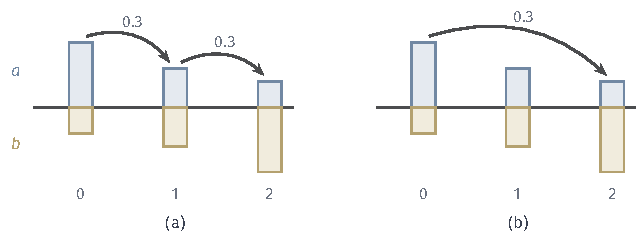
\includegraphics[width=108mm]{figures/07-probability/07-distribution-optimization/tikz/ot-supply-arrows/figure.pdf}
 \caption{全章例子：蓝柱向上是源质量$\bm{a}=(0.5,0.3,0.2)$，黄柱向下是目标质量$\bm{b}=(0.2,0.3,0.5)$，位置为$0,1,2$；箭头上的数是搬运的质量，未画箭头的质量留在原地。(a)逐格搬运，平方成本$0.6$。(b)跳格搬运，平方成本$1.2$。}
 \label{fig:ot-supply-arrows}
\end{BookInlineFigure}

还有许多别的搬法。最“不动脑筋”的是独立搬运：从$x_i$出发的质量按$\bm{b}$的比例分给各个目标，$\pi_{i,j}=a_ib_j$。图~\ref{fig:ot-plan-tables}把三个方案写成表，它们的行和、列和完全相同，平方成本却分别是$1.58$、$1.2$和$0.6$。同一对边缘分布，因质量配对方式不同而产生不同成本；本章的问题就是在全部配对方式中找成本最低的那一个。

\begin{BookInlineFigure}
 \centering
 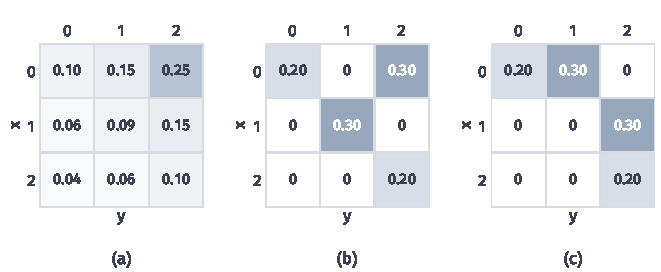
\includegraphics[width=112mm]{figures/07-probability/07-distribution-optimization/matplotlib/ot-plan-tables/figure.pdf}
 \caption{全章例子的三个运输方案，行是源位置$x$，列是目标位置$y$，颜色越深质量越大。三张表的行和都是$\bm{a}$，列和都是$\bm{b}$。(a)独立方案$\pi_{i,j}=a_ib_j$，平方成本$1.58$。(b)跳格搬运，平方成本$1.2$。(c)逐格搬运，平方成本$0.6$。}
 \label{fig:ot-plan-tables}
\end{BookInlineFigure}

这里有三个不同的问题。其一，在全部满足行列约束的方案中优化，允许把一个位置的质量拆开送往几处，这是耦合上的优化。其二，要求每个源位置的质量整体送到一个目标位置，这是运输映射上的优化，可行的方案少得多，甚至可能没有。其三，确认最低成本确实被某个方案取到，而不只是一个无法达到的下确界。下面三小节依次处理。把最低成本当作分布之间的距离时，它的对称性、三角不等式以及与弱收敛的关系已在第~\ref{chap:distribution-comparison}章讨论，本章不再重复。

\subsection{固定边缘的耦合}
\label{sec:ot-couplings}

有限情形的方案是一张非负表。设源有$m$个位置，质量向量$\bm{a}\in\mathbb{R}^{m}$；目标有$n$个位置，质量向量$\bm{b}\in\mathbb{R}^{n}$；两者都非负且总和为$1$。可行方案的全体是
\begin{equation}
 U(\bm{a},\bm{b})=\bigl\{\bm{\pi}\in\mathbb{R}^{m\times n}:\ \bm{\pi}\geq0,\ \bm{\pi}\bm{1}=\bm{a},\ \bm{\pi}^{\top}\bm{1}=\bm{b}\bigr\},
 \label{eq:ot-transport-polytope}
\end{equation}
其中$\bm{\pi}\geq0$指每个元素非负，$\bm{1}$是全一向量。它由有限个线性等式和不等式刻画，是一个有界的凸多面体，称为\term{运输多面体}（transport polytope）。总成本是线性函数
\[
 \langle\bm{C},\bm{\pi}\rangle=\sum_{i,j}c_{i,j}\pi_{i,j} .
\]

把$\bm{\pi}$看成取值于$\{x_i\}\times\{y_j\}$的随机向量$(X,Y)$的联合概率表，行和、列和约束就是“$X$的边缘为$\bm{a}$，$Y$的边缘为$\bm{b}$”，总成本就是$\mathbb{E}[c(X,Y)]$。这正是第~\ref{chap:distribution-comparison}章的耦合：$\mathcal{X}$上的分布$\mu$与$\mathcal{Y}$上的分布$\nu$的耦合是$\mathcal{X}\times\mathcal{Y}$上边缘分别为$\mu,\nu$的分布，全体记作$\Pi(\mu,\nu)$。有限情形$\Pi(\mu,\nu)$与$U(\bm{a},\bm{b})$一一对应。一般情形不再有表，但问题的写法不变。

\begin{definition}[最优运输问题]
\label{def:ot-problem}
设$\mu,\nu$分别是$\mathcal{X},\mathcal{Y}$上的概率分布，$c:\mathcal{X}\times\mathcal{Y}\to[0,\infty]$可测。对耦合$\pi\in\Pi(\mu,\nu)$，称$\int c\,\mathrm{d}\pi$为它的运输成本。称
\begin{equation}
 \operatorname{OT}_c(\mu,\nu)=\inf_{\pi\in\Pi(\mu,\nu)}\int_{\mathcal{X}\times\mathcal{Y}}c(x,y)\,\pi(\mathrm{d}x,\mathrm{d}y)
 \label{eq:ot-kantorovich}
\end{equation}
为\term{最优运输问题}（optimal transport problem）的最优值。耦合也称为\term{运输方案}（transport plan）；达到下确界的耦合称为\term{最优耦合}（optimal coupling）。
\end{definition}

定义要求成本非负，是为了让每个耦合的成本都有意义：非负可测函数的积分总有定义，取值在$[0,\infty]$中，不会出现$\infty-\infty$。若成本有界或下方被可积函数控制，也可以同样处理，但本章只用非负成本。取$\mathcal{X}=\mathcal{Y}$为度量空间、$c=d^{p}$时，$\operatorname{OT}_c^{1/p}$就是第~\ref{chap:distribution-comparison}章的$W_p$。

可行集合从不为空：乘积分布$\mu\otimes\nu$总是一个耦合，它对应“让$X$与$Y$独立”，在有限情形就是图~\ref{fig:ot-plan-tables}(a)的独立方案。但可行不等于有有限成本的方案。取$\mu=\delta_0$，$\nu$为标准Cauchy分布，$c(x,y)=(x-y)^{2}$。$\mu$只有一个点，任何耦合的第一个分量都恒为$0$，所以$\Pi(\mu,\nu)$只有$\delta_0\otimes\nu$一个元素。Cauchy密度与$1/(1+y^{2})$成正比，乘以$y^{2}$后在远处趋于正常数，所以这个唯一耦合的成本是
\[
 \int y^{2}\,\nu(\mathrm{d}y)=\infty .
\]
最优值是$\infty$，问题虽然可行，却给不出任何有用的比较。对$c=\lvert x-y\rvert^{p}$，只要两个分布都有有限$p$阶矩，第~\ref{chap:distribution-comparison}章的估计就说明独立耦合的成本有限；本章讨论的具体问题都满足这类条件。

\subsection{运输映射}
\label{sec:ot-maps}

耦合允许把一个点的质量拆开。如果规定每个源点的质量必须整体送到同一个目标点，方案就由一个函数$T:\mathcal{X}\to\mathcal{Y}$描述：$x$处的质量全部送到$T(x)$。目标处收到的质量分布是$\mu$在$T$下的推前$T_\#\mu$，即$T_\#\mu(B)=\mu(T^{-1}(B))$，推前测度的一般性质可参考\BookChapterRef{chap:pushforward-measures}{卷四第9章“推前测度”}。满足
\begin{equation}
 T_\#\mu=\nu
 \label{eq:ot-transport-map}
\end{equation}
的可测映射称为从$\mu$到$\nu$的\term{运输映射}（transport map）。在映射中优化成本$\int c(x,T(x))\,\mu(\mathrm{d}x)$称为\term{Monge问题}（Monge problem）。

映射是耦合的特例。设$X\sim\mu$，令$Y=T(X)$，则$(X,Y)$的联合分布是
\[
 \pi_T=(\mathrm{id},T)_\#\mu ,
\]
它把全部质量放在$T$的图像$\{(x,T(x))\}$上。它的第一个边缘是$\mu$，第二个边缘是$T_\#\mu=\nu$，所以$\pi_T\in\Pi(\mu,\nu)$，并且$\int c\,\mathrm{d}\pi_T=\mathbb{E}[c(X,T(X))]$。于是Monge问题的下确界不小于$\operatorname{OT}_c(\mu,\nu)$：映射能做的，耦合都能做。

反过来不成立，而且差别可能是根本性的。取$\mu=\delta_0$，$\nu=\tfrac12\delta_{-1}+\tfrac12\delta_1$。任何映射都把$\delta_0$推成单点分布$\delta_{T(0)}$，不可能等于有两个原子的$\nu$，所以映射问题连可行解都没有。耦合问题却有唯一的可行解$\delta_0\otimes\nu$：$0$处的单位质量一分为二，各送一半到$\pm1$，见图~\ref{fig:ot-split-map}(a)。

\begin{BookInlineFigure}
 \centering
 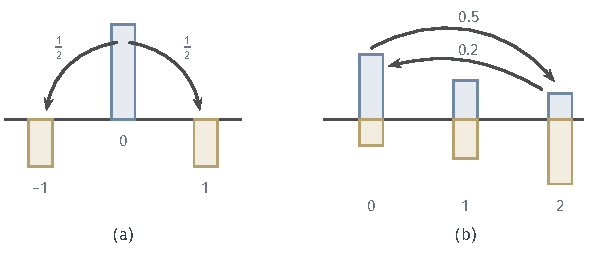
\includegraphics[width=100mm]{figures/07-probability/07-distribution-optimization/tikz/ot-split-map/figure.pdf}
 \caption{映射与耦合。(a)$\delta_0$到$\tfrac12\delta_{-1}+\tfrac12\delta_1$：唯一的耦合把单位质量拆成两半，没有映射能做到。(b)全章例子中唯一的运输映射$T(0)=2$，$T(1)=1$，$T(2)=0$，平方成本$2.8$。}
 \label{fig:ot-split-map}
\end{BookInlineFigure}

全章例子中映射是存在的，但选择极少。$T$把每个源位置的整份质量送到一个目标位置，所以每个$b_j$必须等于若干个$a_i$之和。$b_0=0.2$只能由$a_2=0.2$凑成，$b_1=0.3$只能由$a_1$凑成，剩下$a_0=0.5$正好是$b_2$，于是唯一的映射是$T(0)=2$，$T(1)=1$，$T(2)=0$，平方成本$0.5\cdot4+0.2\cdot4=2.8$，见图~\ref{fig:ot-split-map}(b)。它比逐格搬运的$0.6$贵得多，因为逐格搬运必须把$0$处的$0.5$拆成$0.2$与$0.3$。有限分布之间的映射问题受制于质量能否恰好凑整，耦合问题则没有这个障碍。

\subsection{最优耦合的存在}
\label{sec:ot-existence}

下确界$\operatorname{OT}_c(\mu,\nu)$是否被某个耦合取到？先看有限情形。

\paragraph{有限支持}
运输多面体$U(\bm{a},\bm{b})$非空（含$\bm{a}\bm{b}^{\top}$），是闭集（由等式和非负性定义），并且有界（每个元素在$[0,1]$中），所以是$\mathbb{R}^{m\times n}$中的紧集。成本矩阵各元素有限时，$\langle\bm{C},\bm{\pi}\rangle$是$\bm{\pi}$的连续函数，紧集上的连续函数取到最小值，所以最优方案存在。

图~\ref{fig:ot-polytope}用一个能画出来的例子说明这一点。取$\bm{a}=(0.4,0.6)$位于$x=0,2$，$\bm{b}=(0.2,0.3,0.5)$位于$y=0,1,2$，成本$(x-y)^{2}$。$2\times3$的方案由左上两个元素$s=\pi_{1,1}$、$t=\pi_{1,2}$确定（这里行列下标从$1$起），其余元素是
\[
 \pi_{1,3}=0.4-s-t,\qquad \pi_{2,1}=0.2-s,\qquad \pi_{2,2}=0.3-t,\qquad \pi_{2,3}=0.1+s+t .
\]
非负性给出$0\leq s\leq0.2$，$0\leq t\leq0.3$，$s+t\leq0.4$，这是一个五边形。成本化成
\[
 \langle\bm{C},\bm{\pi}\rangle=t+4(0.4-s-t)+4(0.2-s)+(0.3-t)=2.7-8s-4t ,
\]
等值线是一族平行直线，最小值$0.3$在顶点$(s,t)=(0.2,0.2)$处取得。线性目标在多面体上的最小值总能在顶点处取到，这是线性规划的基本事实，第~\ref{sec:ot-discrete}节还会用到。

\begin{BookInlineFigure}
 \centering
 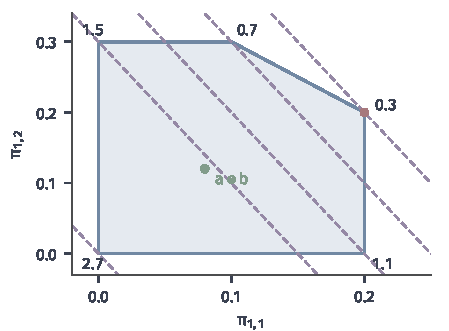
\includegraphics[width=76mm]{figures/07-probability/07-distribution-optimization/matplotlib/ot-polytope/figure.pdf}
 \caption{$\bm{a}=(0.4,0.6)$、$\bm{b}=(0.2,0.3,0.5)$的运输多面体，坐标是$\pi_{1,1}$与$\pi_{1,2}$。浅蓝五边形是可行集，顶点旁的数是该顶点的平方成本；紫色虚线是成本$2.7-8s-4t$的等值线；绿点是独立方案（成本$1.58$），红点是最优顶点（成本$0.3$）。}
 \label{fig:ot-polytope}
\end{BookInlineFigure}

\paragraph{欧氏空间上的分布}
一般分布的耦合集合是无穷维的，需要换一种紧性。第~\ref{chap:weak-convergence-of-distributions}章证明了：$\mathbb{R}^{d}$上一族分布胎紧，则其中任一序列都有弱收敛子列。我们要说明耦合集合正好胎紧，而且弱极限仍是耦合；再说明成本随耦合的变化是下半连续的，即极限处的成本不会突然变大。

\begin{lemma}[耦合集合的紧性]
\label{lem:ot-coupling-compact}
设$\mu,\nu$分别是$\mathbb{R}^{m},\mathbb{R}^{n}$上的概率分布。则$\Pi(\mu,\nu)$胎紧；若$\pi_k\in\Pi(\mu,\nu)$且$\pi_k\xrightarrow{\mathrm{w}}\pi$，则$\pi\in\Pi(\mu,\nu)$。
\end{lemma}

\begin{proof}
任给$\varepsilon>0$。单个分布是胎紧的，取紧集$K_1\subset\mathbb{R}^{m}$与$K_2\subset\mathbb{R}^{n}$，使$\mu(K_1^{\mathrm{c}})<\varepsilon/2$，$\nu(K_2^{\mathrm{c}})<\varepsilon/2$。$K_1\times K_2$是紧集，并且它的补集含于$(K_1^{\mathrm{c}}\times\mathbb{R}^{n})\cup(\mathbb{R}^{m}\times K_2^{\mathrm{c}})$。于是对每个耦合$\pi$，
\[
 \pi\bigl((K_1\times K_2)^{\mathrm{c}}\bigr)\leq\mu(K_1^{\mathrm{c}})+\nu(K_2^{\mathrm{c}})<\varepsilon .
\]
同一个紧集对全部耦合都适用，所以$\Pi(\mu,\nu)$胎紧。

再看弱极限。任取$\mathbb{R}^{m}$上的有界连续函数$h$，函数$(x,y)\mapsto h(x)$在$\mathbb{R}^{m+n}$上有界连续。由弱收敛与第一边缘为$\mu$，
\[
 \int h(x)\,\pi(\mathrm{d}x,\mathrm{d}y)=\lim_{k\to\infty}\int h(x)\,\pi_k(\mathrm{d}x,\mathrm{d}y)=\int h\,\mathrm{d}\mu .
\]
所以$\pi$的第一边缘与$\mu$对一切有界连续函数的积分相同，两者相等。第二边缘同理。
\end{proof}

\begin{lemma}[成本的下半连续性]
\label{lem:ot-cost-lsc}
设$c:\mathbb{R}^{m}\times\mathbb{R}^{n}\to[0,\infty]$是下半连续函数，即对每个点$z$与每个$z_k\to z$有$c(z)\leq\liminf_kc(z_k)$。若概率分布$\pi_k\xrightarrow{\mathrm{w}}\pi$，则
\begin{equation}
 \int c\,\mathrm{d}\pi\leq\liminf_{k\to\infty}\int c\,\mathrm{d}\pi_k .
 \label{eq:ot-cost-lsc}
\end{equation}
\end{lemma}

\begin{proof}
弱收敛只对有界连续函数给出积分的收敛，所以先用有界连续函数从下方逼近$c$。对正整数$j$，令
\[
 c_j(z)=\min\Bigl\{j,\ \inf_{w}\bigl(c(w)+j\lVert z-w\rVert_2\bigr)\Bigr\}.
\]
取$w=z$知$c_j\leq c$；$c_j$关于$j$单调不减，取值在$[0,j]$中。每个$z\mapsto c(w)+j\lVert z-w\rVert_2$都满足$j$-Lipschitz条件，它们的下确界以及与常数$j$的较小者也满足，所以$c_j$连续。

再证$c_j(z)\to c(z)$。任取实数$s<c(z)$。由下半连续，存在$r>0$，使$\lVert w-z\rVert_2<r$时$c(w)>s$。于是对一切$w$，或者$c(w)>s$，或者$j\lVert z-w\rVert_2\geq jr$。当$j\geq\max(s/r,\,s)$时，两种情形下都有
\[
 c(w)+j\lVert z-w\rVert_2\geq s ,
\]
从而$c_j(z)\geq s$。$s$可以任意接近$c(z)$（$c(z)=\infty$时可以任意大），所以$c_j(z)\uparrow c(z)$。

对固定的$j$，$c_j$有界连续，由弱收敛与$c_j\leq c$，
\[
 \int c_j\,\mathrm{d}\pi=\lim_{k\to\infty}\int c_j\,\mathrm{d}\pi_k\leq\liminf_{k\to\infty}\int c\,\mathrm{d}\pi_k .
\]
令$j\to\infty$，由单调收敛定理，左边趋于$\int c\,\mathrm{d}\pi$，得到式~\eqref{eq:ot-cost-lsc}。
\end{proof}

\begin{theorem}[最优耦合的存在]
\label{thm:ot-existence}
设$\mu,\nu$分别是$\mathbb{R}^{m},\mathbb{R}^{n}$上的概率分布，$c:\mathbb{R}^{m}\times\mathbb{R}^{n}\to[0,\infty]$下半连续。则存在$\pi^{*}\in\Pi(\mu,\nu)$，使
\begin{equation}
 \int c\,\mathrm{d}\pi^{*}=\operatorname{OT}_c(\mu,\nu).
 \label{eq:ot-existence}
\end{equation}
\end{theorem}

\begin{proof}
若$\operatorname{OT}_c(\mu,\nu)=\infty$，每个耦合都达到它。下设它有限，取耦合列$\pi_k$，使其成本递减地趋于$\operatorname{OT}_c(\mu,\nu)$。由引理~\ref{lem:ot-coupling-compact}，这列耦合胎紧，由第~\ref{chap:weak-convergence-of-distributions}章的弱收敛子列定理，存在子列$\pi_{k_l}\xrightarrow{\mathrm{w}}\pi^{*}$，并且$\pi^{*}\in\Pi(\mu,\nu)$。由引理~\ref{lem:ot-cost-lsc}，
\[
 \int c\,\mathrm{d}\pi^{*}\leq\liminf_{l\to\infty}\int c\,\mathrm{d}\pi_{k_l}=\operatorname{OT}_c(\mu,\nu).
\]
反向不等式由下确界的定义成立。
\end{proof}

定理的两个条件各有分工。固定边缘使耦合集合胎紧，这是“极小化序列有收敛子列”的来源；下半连续使成本在极限处不会跳高，这是“极限仍是最小者”的来源。$\mathbb{R}^{d}$可以换成一般的完备可分度量空间，证明相同，只是要用一般形式的Prokhorov定理，可查阅~\scite{math-villani2009transport}。

\paragraph{去掉下半连续性}
下面的例子说明下半连续不能省。取$\mu=\nu=\operatorname{Unif}(0,1)$，成本在对角线上取$1$，在对角线外取距离：
\[
 c(x,y)=\begin{cases}1, & x=y,\\ \lvert x-y\rvert, & x\neq y .\end{cases}
\]
它在对角线上不是下半连续的：$c(x,x)=1$，而附近的$c(x,x+h)=\lvert h\rvert\to0$。对$0<h<1$，令$X\sim\operatorname{Unif}(0,1)$，$Y=X+h$（若超过$1$则减去$1$）。$Y$仍服从$\operatorname{Unif}(0,1)$，$X\neq Y$，并且$\lvert X-Y\rvert$以概率$1-h$等于$h$、以概率$h$等于$1-h$，所以成本是
\[
 (1-h)h+h(1-h)=2h(1-h)\to0\qquad(h\to0).
\]
于是$\operatorname{OT}_c(\mu,\nu)=0$。但没有耦合的成本为$0$：若$\pi$在对角线上有正质量，成本至少是这部分质量；若没有，$\pi$的质量全在$\{x\neq y\}$上，$\lvert x-y\rvert>0$处处成立，积分为正。极小化序列弱收敛到对角线上的耦合，成本却在极限处跳到$1$。

\paragraph{耦合存在而映射不达到}
定理只保证最优耦合存在。即使最优耦合存在，Monge问题的下确界也可能取不到。在$\mathbb{R}^{2}$中取$\mu$为线段$\{0\}\times[0,1]$上的均匀分布，$\nu$把一半质量均匀放在$\{-1\}\times[0,1]$上，另一半均匀放在$\{1\}\times[0,1]$上，成本为平方欧氏距离。任何耦合都要把每份质量横向移动距离$1$，所以成本至少为$1$；把每个点的质量平分到左右两侧同一高度，成本恰为$1$，是最优耦合。

映射却做不到$1$。把$[0,1]$等分成$n$段，每段的下半段水平送到左侧、上半段送到右侧，并在竖直方向拉伸两倍铺满该段，得到映射$T_n$。竖直位移在每半段上均匀分布在长为$1/(2n)$的区间里，平均平方为$1/(12n^{2})$，所以$T_n$的成本是
\[
 1+\frac{1}{12n^{2}}\to1 ,
\]
见图~\ref{fig:ot-monge-stripes}。若某个映射$T$的成本恰为$1$，竖直位移必须几乎处处为零，即$T(0,s)=(\pm1,s)$。记$L$为送往左侧的高度集合，左侧收到的质量中高度落在$L$里的部分是$\lvert L\rvert$，而$\nu$要求它是$\lvert L\rvert/2$，所以$\lvert L\rvert=0$；左侧总共却必须收到$1/2$，矛盾。

\begin{BookInlineFigure}
 \centering
 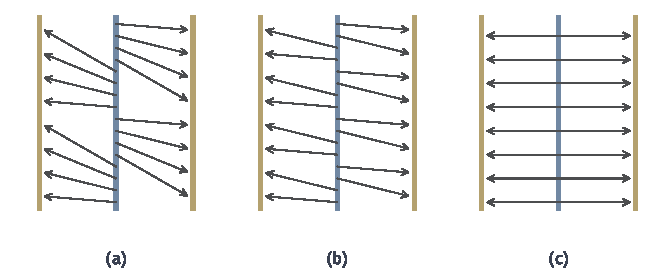
\includegraphics[width=112mm]{figures/07-probability/07-distribution-optimization/matplotlib/ot-monge-stripes/figure.pdf}
 \caption{蓝色竖线是$\mu$（$\{0\}\times[0,1]$上均匀），两条黄色竖线各带$\nu$的一半质量。(a)$n=2$的条带映射$T_2$，成本$1+1/48$。(b)$n=4$的条带映射，成本$1+1/192$。(c)最优耦合把每个点的质量平分到两侧，成本$1$，任何映射都达不到。}
 \label{fig:ot-monge-stripes}
\end{BookInlineFigure}

所以“最优方案存在”只针对耦合。最优耦合能否由映射实现，以及是否唯一，都要另加条件，第~\ref{sec:ot-concrete}节会在具体问题中看到这些条件。
